%% Springer Nature — Math and Physical Sciences Numbered Reference Style
%% Paper: "A Deterministic Wavefunction-Token Cascade Architecture for
%%         Monte Carlo Matrix Element Evaluation on AMD Versal AI Engines"
%%
%% NOTE: Copy sn-jnl.cls and the bst/ folder from springer_template/ here,
%%       or adjust \documentclass path accordingly.
%%
\documentclass[pdflatex,sn-mathphys-num,iicol]{sn-jnl}

%%%% Packages
\usepackage{graphicx}
\graphicspath{{figures/}}
\usepackage{multirow}
\usepackage{amsmath,amssymb,amsfonts}
\usepackage{mathrsfs}
\usepackage{booktabs}
\usepackage{xcolor}
\usepackage{xspace}
\usepackage{listings}
\usepackage{algorithm}
\usepackage{algorithmicx}
\usepackage{algpseudocode}
\usepackage{siunitx}
\usepackage{subcaption}
\usepackage[title]{appendix}

%%%% Custom commands (process/physics shorthands)
\newcommand{\hilumi}{HL-LHC\xspace}
\newcommand{\amcnlo}{\textsc{MadGraph5\_aMC@NLO}\xspace}
\newcommand{\mgfive}{MG5aMC\xspace}
\newcommand{\ttbar}{\ensuremath{\mathrm{t}\bar{\mathrm{t}}}\xspace}
\newcommand{\gluglu}{\ensuremath{\mathrm{gg}}\xspace}
\newcommand{\ggtt}{\ensuremath{\gluglu\rightarrow\ttbar}\xspace}
\newcommand{\ggttg}{\ensuremath{\gluglu\rightarrow\ttbar\,\mathrm{g}}\xspace}
\newcommand{\ME}{$|{\cal M}|^2$\xspace}
\newcommand{\jamp}{\texttt{JAMP}\xspace}
\newcommand{\aie}{AI Engine\xspace}
\newcommand{\aies}{AI Engines\xspace}
\newcommand{\KB}{\,\text{KB}\xspace}
\newcommand{\TODO}[1]{\textcolor{red}{\textbf{[TODO: #1]}}}

%%%% Theorem styles (required by sn-jnl.cls)
\theoremstyle{thmstyleone}
\newtheorem{theorem}{Theorem}
\newtheorem{proposition}[theorem]{Proposition}
\theoremstyle{thmstyletwo}
\newtheorem{example}{Example}
\newtheorem{remark}{Remark}
\theoremstyle{thmstylethree}
\newtheorem{definition}{Definition}

\raggedbottom

\begin{document}

%% ─── Title ───────────────────────────────────────────────────────────────────
\title[Wavefunction-Token Cascade for MC Matrix Elements on AMD Versal AI Engines]%
{A Deterministic Wavefunction-Token Cascade Architecture\\
for Monte Carlo Matrix Element Evaluation\\
on AMD Versal AI Engines}

%% ─── Authors ─────────────────────────────────────────────────────────────────
\author*[1]{\fnm{J.}  \sur{Fern\'{a}ndez Men\'{e}ndez}}\email{jfm@uniovi.es}
\author[2]{\fnm{L.}   \sur{Fiorini}}
\author[1]{\fnm{S.}   \sur{Folgueras}}
\author[2]{\fnm{F.}   \sur{Herv\'{a}s \'{A}lvarez}}
\author[2]{\fnm{H.}   \sur{Guti\'{e}rrez Arance}}
\author[1]{\fnm{P.}   \sur{Leguina L\'{o}pez}}
\author[2]{\fnm{A.}   \sur{Oyanguren}}
\author[2]{\fnm{A.}   \sur{Valero}}
\author[3]{\fnm{C.}   \sur{Vico Villalba}}

\affil*[1]{\orgname{Universidad de Oviedo -- ICTEA},
           \orgaddress{\city{Oviedo}, \country{Spain}}}
\affil[2]{\orgname{Instituto de F\'{i}sica Corpuscular (IFIC)},
          \orgdiv{Universitat de Val\`{e}ncia -- CSIC},
          \orgaddress{\city{Valencia}, \country{Spain}}}
\affil[3]{\orgname{Rice University},
          \orgaddress{\city{Houston}, \state{Texas}, \country{USA}}}

%% ─── Abstract ────────────────────────────────────────────────────────────────
\abstract{%
We present a deterministic wavefunction-token cascade architecture for
accelerating leading-order Monte Carlo matrix element evaluation on AMD Versal
\aie arrays.  Targeting the \ggttg process generated by \amcnlo, we address
the fundamental constraint that the 16~Feynman diagrams and associated HELAS
routines required for this process exceed the 16\KB program memory of a single
\aie tile by a factor of ${\sim}2.4\times$.  We introduce a
program-memory-driven partitioning methodology that decomposes the monolithic
computation into a five-kernel cascade pipeline (\texttt{K1}--\texttt{K4}),
where each kernel fits within the hardware limit while preserving physics
equivalence.  Inter-kernel communication is carried over the deterministic
384-bit cascade interface via a novel wavefunction-token protocol transferring
external wavefunctions, VVV propagator products, and partially accumulated
colour-flow amplitudes (JAMP) between tiles at 48\,GB/s.  We formalise the
cascade contract---requiring identical loop skeletons across all kernels in a
pipeline---that guarantees deadlock-free operation without flow control.  A
lazy-evaluation optimisation for the \texttt{FFV1P0\_3} vertex reduces the
bottleneck kernel's program memory from 17.8\KB to 15.5\KB, eliminating the
last overflow.  The architecture scales to 80~parallel pipelines across the
400-tile \aie array using native packet switching
($10\times\texttt{pktsplit}\langle 8\rangle$), achieving 100\% tile
utilisation.  Physics equivalence is validated at the JAMP level against the
\mgfive reference implementation, confirming identical diagram-by-diagram
amplitude accumulation.
}

\keywords{Monte Carlo event generation, Versal AI Engine, matrix element acceleration, cascade pipeline, HELAS, FPGA}

\maketitle

%% ─── Sections ────────────────────────────────────────────────────────────────
%% sec_introduction.tex
%% ─────────────────────────────────────────────────────────────────────────────
%% Section 1 — Introduction
%% ─────────────────────────────────────────────────────────────────────────────

\section{Introduction}\label{sec:intro}

Due to the intrinsically probabilistic nature of fundamental particle
interactions and the composite structure of the proton, accurately modelling
the dynamics of proton collisions at the Large Hadron Collider (LHC)
constitutes one of the major challenges in high-energy physics
(HEP)~\cite{HSFPhysicsEventGeneratorWG:2020gxw}.  Physics event generators
encode the necessary theoretical tools in computational form, enabling
quantitative predictions for a given model and process via Monte Carlo (MC)
techniques.

For a given process, the generator samples a large number of random
phase-space points (PSPs) and evaluates the squared matrix element \ME at each
point.  As the LHC moves into its High-Luminosity phase (\hilumi), the
simulation demand grows super-linearly while the computing budget remains
flat---a gap that cannot be closed by conventional CPU improvements
alone~\cite{HSFPhysicsEventGeneratorWG:2020gxw}.  The matrix element (ME)
evaluation step is the dominant computational bottleneck, accounting for
30--40\% of total generator CPU time in multi-jet processes~\cite{Valassi:2021ljk}.

This bottleneck has driven substantial parallelism efforts.  The \amcnlo
(\mgfive) CUDACPP plugin~\cite{Valassi:2025xfn} exploits GPU and
vectorised-CPU architectures to deliver speedups of
$100\times$--$1000\times$ over single-threaded Fortran on complex processes.
Field-Programmable Gate Arrays (FPGAs) offer an orthogonal route: custom
fixed-function datapaths designed around the exact computation required, with
typically far lower power consumption than GPUs.  Barbone et
al.~\cite{Carrazza:2021gpx} demonstrated a ${\sim}100\times$ CPU speedup for
the $e^+e^-\to\mu^+\mu^-$ matrix element on a Xilinx Alveo card.  The AMD
Versal Adaptive Compute Acceleration Platform (ACAP) extends this further by
co-integrating a programmable logic (PL) fabric with an array of specialised
\aie cores~\cite{Barbone:2023mul}.

In this paper we describe the first full-array implementation of a
leading-order ME pipeline on the Versal VCK190, targeting the
\ggttg process generated by \mgfive.  Our central contribution is an
\textit{architectural} one: we show how the 16\KB program-memory (PM) limit of
a single \aie tile fundamentally constrains the design, and we present a
systematic methodology---driven by per-function PM profiling, a formal cascade
contract, and a novel wavefunction-token protocol---that maps the complete
16-diagram \ggttg computation onto 80 parallel cascade pipelines occupying all
400 \aie tiles of the device.

The specific contributions of this work are:
\begin{enumerate}
  \item \textbf{Wavefunction-token cascade pipeline architecture.}
    A five-stage pipeline (\texttt{K1}$\to$\texttt{K2a}$\to$\texttt{K2b}%
    $\to$\texttt{K3}$\to$\texttt{K4}) that decomposes 16 Feynman diagrams
    across five \aie tiles.  Tiles communicate via a 384-bit cascade token
    carrying external wavefunctions, precomputed VVV propagators, and partial
    JAMP accumulators.

  \item \textbf{Program-memory-driven partitioning methodology.}
    We profile every HELAS function's PM footprint, derive the \textit{VVV
    Exclusion Principle} (\texttt{VVV1P0\_1} and \texttt{VVV1\_0} cannot
    coexist in one tile), and apply a lazy-evaluation optimisation that moves
    \texttt{FFV1P0\_3} from \texttt{K1} to \texttt{K3}, eliminating the last
    PM overflow.

  \item \textbf{Deterministic cascade contract.}
    Formal rules---all kernels share the same \texttt{BATCH}$\times$32 loop
    skeleton; cascade writes are unconditional; token counts are statically
    matched---that guarantee deadlock-free operation without flow-control
    hardware.

  \item \textbf{HELAS-to-AIE adaptation.}
    Porting of the full MadGraph HELAS library to \texttt{aie::vector<cfloat,8>}
    intrinsics, including complex-division elimination, vectorised spinor cores,
    and binary-indexed helicity caching.

  \item \textbf{Scalable packet-switched array and full PS--PL--AIE system.}
    Scale-up to 80 independent pipelines via
    $10\times\texttt{pktsplit}\langle 8\rangle$, embedded in a three-layer
    system: ARM A72 PS (RAMBO phase-space generation + XRT), PL (10$\times$ HLS
    MM2S/S2MM data movers), and the \aie array.

  \item \textbf{Physics equivalence validation.}
    Diagram-by-diagram JAMP comparison against the \mgfive double-precision
    reference, documenting the float32 tolerance.
\end{enumerate}

The remainder of the paper is structured as follows.
Section~\ref{sec:background} reviews \mgfive and the \ggttg process.
Section~\ref{sec:platform} describes the Versal VCK190 target hardware.
Section~\ref{sec:architecture} presents the cascade pipeline architecture.
Section~\ref{sec:implementation} details the HELAS adaptation and system
integration.
Section~\ref{sec:results} reports program-memory, precision, throughput, and
energy results.
Section~\ref{sec:conclusion} concludes and discusses future directions.

%% sec_background.tex
%% ─────────────────────────────────────────────────────────────────────────────
%% Section 2 — Background and Related Work
%% ─────────────────────────────────────────────────────────────────────────────

\section{Background and Related Work}\label{sec:background}

\subsection{MC event generation and the matrix element bottleneck}

Physics event generators model proton collisions by integrating the transition
probability
\begin{equation}
  \mathcal{P}(i\to\mathcal{X})
  = \left|\mathcal{M}_{i\to\mathcal{X}}\right|^2,
  \label{eq:me}
\end{equation}
over phase space using MC sampling.  The calculation is \emph{embarrassingly
parallel}: the same \ME evaluation is performed independently for each sampled
PSP.  Modern generators such as \amcnlo provide automatic generation of the
amplitude code from Feynman rules via the HELAS
library~\cite{Murayama:1992gi}, where each diagram corresponds to a sequence
of wavefunction and vertex calls accumulating into colour-flow amplitude sums
(\jamp).

\subsection{\ggttg as validation benchmark}\label{sec:process}

We target the \ggttg process at leading order.  \mgfive generates 16 Feynman
diagrams ($\mathrm{D1}$--$\mathrm{D16}$, where $\mathrm{D16}$ has three
sub-diagrams via four-gluon contact vertices), 6 colour-flow amplitudes
($\jamp[0..5]$), and 32 helicity configurations.  The complete HELAS call
graph involves 10 distinct functions:
\texttt{ixxxxx}, \texttt{oxxxxx}, \texttt{vxxxxx} (external wavefunctions);
\texttt{FFV1\_0/1/2}, \texttt{FFV1P0\_3} (fermion--fermion--vector vertices);
\texttt{VVV1P0\_1}, \texttt{VVV1\_0} (triple-gluon vertices);
\texttt{VVVV1/3/4P0\_1} (four-gluon contact vertices).

Although the process is relatively compact (5 external particles), it provides
a demanding PM stress-test: the monolithic kernel implementing all 16 diagrams
requires ${\sim}38\KB$ of program memory---$2.4\times$ the 16\KB tile limit.
This makes \ggttg the minimal realistic benchmark for the partitioning
methodology developed here.

\subsection{GPU and vectorised-CPU acceleration}

The CUDACPP plugin for \mgfive~\cite{Valassi:2025xfn} achieves
$100\times$--$1000\times$ speedup over single-threaded Fortran on NVIDIA V100
GPUs for processes such as $\gluglu\to\ttbar\gluglu\gluglu$.  CPU vector
implementations (AVX2/AVX-512) deliver up to $16\times$ on a single core.
These results establish the performance target against which the AIE
architecture is compared in Section~\ref{sec:results}.

\subsection{Prior FPGA acceleration work}

Barbone et al.~\cite{Carrazza:2021gpx} demonstrated ${\sim}100\times$ CPU
speedup for $e^+e^-\to\mu^+\mu^-$ on a Xilinx Alveo using HLS-generated
circuits.  Barbone et al.~\cite{Barbone:2023mul} subsequently extended this to
the Versal platform, combining PL HLS kernels, VHDL datapaths, and \aie
kernels for the same two-body process.  Our work differs in two key respects:
(i)~we target a significantly more complex hadronic process (\ggttg with 16
diagrams vs.\ 1--2 for $e^+e^-\to\mu^+\mu^-$), and (ii)~we identify PM
constraints as the primary architectural driver, motivating a multi-tile
cascade pipeline rather than a single-core solution.

%% sec_platform.tex
%% ─────────────────────────────────────────────────────────────────────────────
%% Section 3 — Target Platform: AMD Versal AI Engine Architecture
%% ─────────────────────────────────────────────────────────────────────────────

\section{Target Platform: AMD Versal AI Engine Architecture}\label{sec:platform}

\subsection{Device overview}

The AMD Versal AI Core Series VCK190 evaluation kit is built around the
XCVC1902 Adaptive Compute Acceleration Platform (ACAP).  The device integrates
three compute domains on a single die: a dual-core ARM Cortex-A72 application
processor (1.7\,GHz) used for system control and host orchestration; a
dual-core ARM Cortex-R5F real-time processor; and the programmable logic (PL)
fabric with 899\,840 LUTs, 1\,968 DSP58 engines, and 158\,MB of embedded
memory (UltraRAM + BRAM).  The AI Engine array is the key resource for
computation in this work.

\subsection{AI Engine tile microarchitecture}\label{sec:aie_tile}

The device contains \textbf{400 \aie tiles} arranged in a $50\times 8$ array
and clocked at 1\,GHz.  Each tile comprises:
\begin{itemize}
  \item A 512-bit SIMD vector unit supporting single-precision (float32) and
    fixed-point arithmetic;
  \item A 32-bit scalar RISC core for control flow;
  \item 32\,KB of local data memory (plus 128\,KB addressable via neighbours);
  \item \textbf{16\,KB of dedicated program memory (PM)}---the hard constraint
    that drives the architecture of this work.
\end{itemize}

\subsection{Cascade interface}\label{sec:cascade}

Adjacent tiles in the same row are connected by a \textbf{cascade interface}:
a 384-bit unidirectional accumulator bus clocked in lock-step with the vector
pipeline.  Key properties relevant to this work are:
\begin{itemize}
  \item \textbf{Deterministic, zero-overhead data transfer}: one 384-bit word
    ($4\times\texttt{cfloat}$) per clock cycle, no flow-control signals.
  \item \textbf{Hardware FIFO}: a 4-entry FIFO decouples producer and consumer
    by up to 4 cycles, absorbing minor skew without stalling.
  \item \textbf{Fixed direction per row}: even rows (0, 2, 4, 6) cascade
    left-to-right; odd rows (1, 3, 5, 7) cascade right-to-left.  Kernel
    placement must match this hardware topology.
  \item \textbf{Bandwidth}: $384\,\text{bits}/\text{cycle} \times 1\,\text{GHz}
    = 48\,\text{GB/s}$, far exceeding the stream I/O bandwidth from the shim.
\end{itemize}

\subsection{Stream switching and PLIO}

Tiles communicate with the PL through \emph{Programmable Logic I/O} (PLIO)
ports at the shim row.  On XCVC1902, valid shim columns for PLIO placement are
columns 6--43 (columns 0--5 and above 43 host AIE-PL interface tiles but not
direct PLIO sites).  The stream switch network routes packets between tiles
using packet headers, enabling \texttt{pktsplit} and \texttt{pktmerge}
primitives that distribute or collect one stream to/from multiple tiles without
dedicated PL logic.

\subsection{Program memory as the primary constraint}

Unlike GPU or CPU codebases where code size is virtually unconstrained, the
16\KB PM limit is hard and non-negotiable.  A kernel that overflows PM cannot
be compiled.  Table~\ref{tab:pm_footprint} quantifies the PM contribution of
each HELAS function used in \ggttg, establishing why no single tile can hold
the complete computation.

\begin{table}[h]
\caption{Estimated program memory footprint of each HELAS function used for
\ggttg on the \aie.  Values are representative; exact figures depend on
compiler optimisation flags.  The 16\KB hardware limit is shown for
reference.}
\label{tab:pm_footprint}
\begin{tabular}{@{}lrl@{}}
\toprule
HELAS function / component & PM (bytes) & Used in \\
\midrule
\texttt{VVV1P0\_1} (off-shell gluon)          & ${\sim}2{,}000$ & K1 \\
\texttt{FFV1P0\_3} (off-shell boson)          & ${\sim}2{,}700$ & K3 (moved) \\
\texttt{FFV1\_0/1/2} (FFV amplitudes)         & ${\sim}4{,}400$ & K2a, K2b \\
\texttt{VVV1\_0} (triple-gluon amplitude)     & ${\sim}2{,}100$ & K3 \\
\texttt{VVVV1/3/4P0\_1} (4-gluon contact)    & ${\sim}6{,}600$ & K4 \\
Kernel logic + token serialisation            & ${\sim}11{,}000$ & all \\
Softfloat runtime                             & ${\sim}1{,}500$ & all \\
\midrule
\textbf{Monolithic total}                     & ${\sim}38{,}000$ & --- \\
\textbf{16\KB hardware limit}                 & $16{,}384$ & --- \\
\bottomrule
\end{tabular}
\end{table}

The \textbf{VVV Exclusion Principle} emerges directly from
Table~\ref{tab:pm_footprint}: \texttt{VVV1P0\_1} (${\sim}2.0\KB$) and
\texttt{VVV1\_0} (${\sim}2.1\KB$), when combined with the kernel logic
overhead, cannot coexist in a single 16\KB tile.  They must reside in
separate kernels---\texttt{K1} and \texttt{K3} respectively.

%% sec_architecture.tex
%% ─────────────────────────────────────────────────────────────────────────────
%% Section 4 — Wavefunction-Token Cascade Architecture
%% ─────────────────────────────────────────────────────────────────────────────

\section{Wavefunction-Token Cascade Architecture}\label{sec:architecture}

\subsection{Pipeline overview}

The complete \ggttg matrix element computation is decomposed into a
\textbf{five-kernel cascade pipeline} spanning five consecutive \aie tiles in
a single row:
\begin{equation}
  \underbrace{\texttt{K1}}_{\text{WFGEN}}
  \xrightarrow{\text{8-WF token}}
  \underbrace{\texttt{K2a}}_{\text{FF\_DIAG\_A}}
  \xrightarrow{\text{8-WF token}}
  \underbrace{\texttt{K2b}}_{\text{FF\_DIAG\_B}}
  \xrightarrow{\text{8-WF token}}
  \underbrace{\texttt{K3}}_{\text{VVV\_AMP}}
  \xrightarrow{\text{5-WF token}}
  \underbrace{\texttt{K4}}_{\text{VVVV\_COLOR}}
  \label{eq:pipeline}
\end{equation}
Only the boundary kernels (\texttt{K1} and \texttt{K4}) have stream I/O; all
interior kernels are purely cascade-in/cascade-out.  This clean separation
means the cascade pipeline design is independent of the I/O topology.

\begin{figure*}[t]
\centering
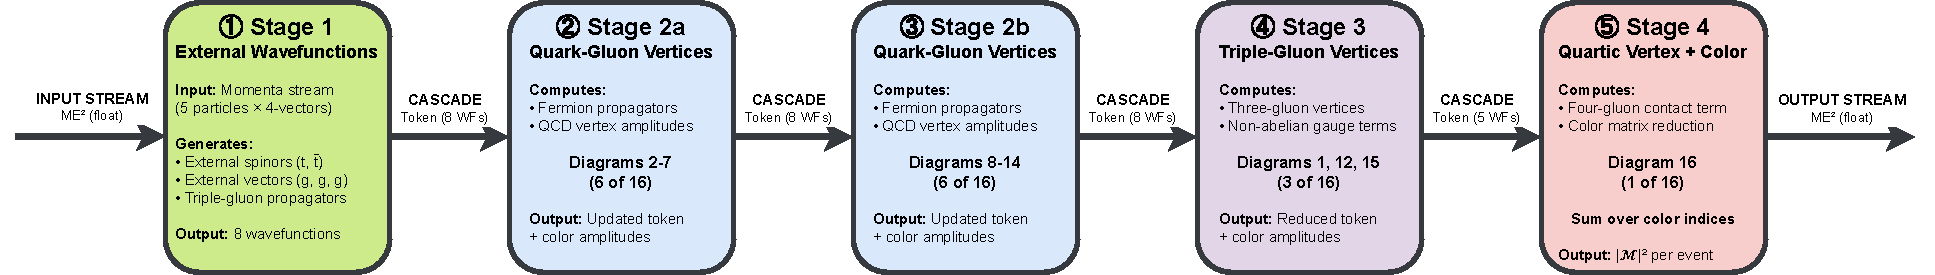
\includegraphics[width=\textwidth]{Fig1}
\caption{\textbf{Fig.\,1} Single cascade pipeline (one row of 5 AIE tiles).
  Stage~1 (K1, WFGEN) receives the input PSP packet stream, generates 8 external
  wavefunctions, and transmits an 8-WF token over the cascade bus.
  Stages~2a and 2b (K2a/K2b) evaluate fermion-loop quark-gluon diagrams D2--D7
  and D8--D14 respectively, accumulating colour-flow amplitudes (JAMP) into the
  token.  Stage~3 (K3, VVV\_AMP) handles triple-gluon vertex diagrams D1, D12,
  and D15, reducing the token width from 8~WFs to 5~WFs.  Stage~4 (K4,
  VVVV\_COLOR) computes the four-gluon contact diagram D16 and performs the
  colour-matrix reduction, emitting the scalar ME$^2$ result as an output
  packet stream.  Cascade labels show token type (8-WF or 5-WF) and the
  cascade bus width is 384~bits at 1.25~GHz.}
\label{fig:single_pipe}
\end{figure*}

\subsection{Diagram-to-kernel assignment}\label{sec:diagram_assign}

Table~\ref{tab:diag_assign} shows which Feynman diagrams are evaluated in each
kernel and which HELAS functions are required.

\begin{table}[h]
\caption{Diagram-to-kernel assignment for \ggttg.  D16 has three
sub-diagrams (a, b, c) using four-gluon contact vertices.  D12 is evaluated
in K3 alongside the triple-gluon diagrams because its required vertex
\texttt{VVV1\_0} resides there.}
\label{tab:diag_assign}
\begin{tabular}{@{}llll@{}}
\toprule
Kernel & Diagrams & Key HELAS functions & JAMP contribution \\
\midrule
K1 & --- (wavefunction generation) &
  \texttt{ixxxxx}, \texttt{oxxxxx}, \texttt{vxxxxx}, \texttt{VVV1P0\_1}
  & initialise to 0 \\
K2a & D2, D3, D4, D5, D6, D7 &
  \texttt{FFV1\_0/1/2}
  & accumulate \\
K2b & D8, D9, D10, D11, D13, D14 &
  \texttt{FFV1\_0/1/2}
  & accumulate \\
K3 & D1, D12, D15 &
  \texttt{FFV1P0\_3}, \texttt{VVV1\_0}
  & accumulate \\
K4 & D16a, D16b, D16c &
  \texttt{VVVV1/3/4P0\_1}, \texttt{FFV1\_0}
  & accumulate + colour reduction \\
\bottomrule
\end{tabular}
\end{table}

\subsection{Token design}\label{sec:token}

All inter-kernel state is passed via a \emph{cascade token}---a structured
sequence of cascade beats encoding wavefunctions and the partial JAMP
accumulator.  Two token formats are used:

\paragraph{Extended 8-WF token (K1$\to$K2a$\to$K2b$\to$K3).}
Contains five external wavefunctions ($w_0$--$w_4$) plus three precomputed VVV
propagators ($w_{5,01} = \texttt{VVV1P0\_1}(w_0,w_1)$,
$w_{10} = \texttt{VVV1P0\_1}(w_1,w_4)$,
$w_{5,04} = \texttt{VVV1P0\_1}(w_0,w_4)$), and JAMP[6]:
\begin{equation}
  \underbrace{8 \times 2\ \text{beats}}_{\text{wavefunctions}}
  +\ \underbrace{2\ \text{beats}}_{\text{JAMP}[6]}
  = 18\ \text{cascade beats per helicity}.
  \label{eq:extended_token}
\end{equation}
Each beat transfers $4\times\texttt{cfloat} = 8$ single-precision complex
values (32\,bytes) via the 384-bit accumulator.  Wavefunctions use 6 of 8
lanes (lanes~0--5 carry the physics values; lanes~6--7 are zero-padded).

\paragraph{Standard 5-WF token (K3$\to$K4).}
Contains only the five external wavefunctions plus JAMP[6]:
\begin{equation}
  5 \times 2 + 2 = 12\ \text{cascade beats per helicity}.
  \label{eq:standard_token}
\end{equation}
K3 computes \texttt{FFV1P0\_3}$(w_3, w_2)$ locally and does not need to
forward it, reducing the token by 3 wavefunctions.

\subsection{Redundant propagator recomputation as a design choice}
\label{sec:redundant_recompute}

K2a and K2b each independently compute the same six propagators
($w_7, w_8, w_9, w_{5,20}, w_{5,30}, w_{11}$) from the external wavefunctions
carried in the token.  This is deliberate: passing the 6 propagators in the
token would require 12 additional cascade beats per helicity iteration,
increasing token size by 67\%.  If instead each propagator is recomputed
at a cost of ${\sim}200$ cycles, the cascade remains at 18 beats and tile
bandwidth is reduced by ${\sim}40\%$.  This computation-vs-communication
trade-off is central to keeping the architecture pipeline-bound rather than
cascade-bound.

\subsection{Deterministic cascade contract}\label{sec:contract}

To guarantee deadlock-free operation, all kernels in a pipeline must obey the
\textbf{cascade contract}:
\begin{enumerate}
  \item \textbf{Identical loop skeletons}: every kernel executes exactly
    \texttt{for (b in 0..BATCH) \{ for (h in 0..31) \{ ... \} \}}.  No early
    exits, no data-dependent iteration counts.
  \item \textbf{Unconditional cascade writes}: every iteration writes exactly
    one token to the cascade.  Conditional writes cause FIFO drift between
    adjacent tiles, eventually causing deadlock.
  \item \textbf{Statically matched counts}: the compiler-visible token
    write/read counts are equal across every producer/consumer pair at compile
    time.
\end{enumerate}
These rules are enforced by the token API implemented in
\texttt{kernels\_4k\_token.h}, which provides \texttt{write\_token\_8wf\_k1},
\texttt{read\_token\_8wf\_k1}, \texttt{write\_token\_5wf}, and
\texttt{read\_token\_5wf} as the only legal inter-kernel communication
primitives.

The 4-entry hardware FIFO on the cascade link absorbs minor cycle-to-cycle
timing skew (e.g., from branch mispredictions in the scalar unit) as long as
the loop-skeleton structure is preserved.

\subsection{Scalable 80-pipeline array architecture}\label{sec:array}

\paragraph{Group and row layout.}
The 400 \aie tiles are organised as $10\ \text{groups} \times 8\ \text{rows}$
$= 80$ pipelines.  Group~$g$ occupies columns $[5g, 5g+4]$; the five kernels
(\texttt{K1}--\texttt{K4}) occupy exactly those five columns.

\paragraph{Cascade direction compliance.}
Even rows cascade left-to-right; odd rows right-to-left.  Accordingly:
\begin{itemize}
  \item Even row $r$: \texttt{K1} at column $5g$, \texttt{K4} at $5g+4$.
  \item Odd row $r$: \texttt{K1} at column $5g+4$, \texttt{K4} at $5g$.
\end{itemize}
The HELAS kernel bodies are identical for all 80 pipelines; only the ADF
placement constraints differ.

\paragraph{Packet switching.}
Each group $g$ is served by one PLIO pair pinned to shim column $4g+6$
(giving columns 6, 10, 14, \ldots, 42---all valid shim sites on XCVC1902).  A
$\texttt{pktsplit}\langle 8\rangle$ node fans the incoming stream to all 8
\texttt{K1} tiles in the group (one per row); a $\texttt{pktmerge}\langle
8\rangle$ node collects all 8 \texttt{K4} outputs.  Packet ID bits
$[4:0]$ of the header encode the row index (0--7), routing each PSP to the
correct pipeline.  With 10 groups, the full array uses $10$ PLIO input pairs and
$10\times\texttt{pktsplit}\langle 8\rangle$.

\paragraph{Full-system three-layer stack.}
\begin{itemize}
  \item \textbf{PS (ARM A72)}: RAMBO phase-space generator produces PSPs;
    XRT runtime manages XCLBIN loading, buffer allocation, and synchronisation.
  \item \textbf{PL}: 10$\times$ HLS \texttt{MM2S\_pkt\_gen} kernels read PSP
    arrays from DDR and generate packet-headered AXI-Stream at II=1 (32-bit,
    500\,MHz).  10$\times$ HLS \texttt{S2MM\_pkt\_parser} collect
    \texttt{pktmerge} output and write ME$^2$ results to DDR.
  \item \textbf{AIE array}: 80 independent five-tile cascade pipelines
    consuming \texttt{input\_pktstream} in \texttt{K1} and emitting
    \texttt{output\_pktstream} from \texttt{K4}.
\end{itemize}

\begin{figure*}[t]
\centering
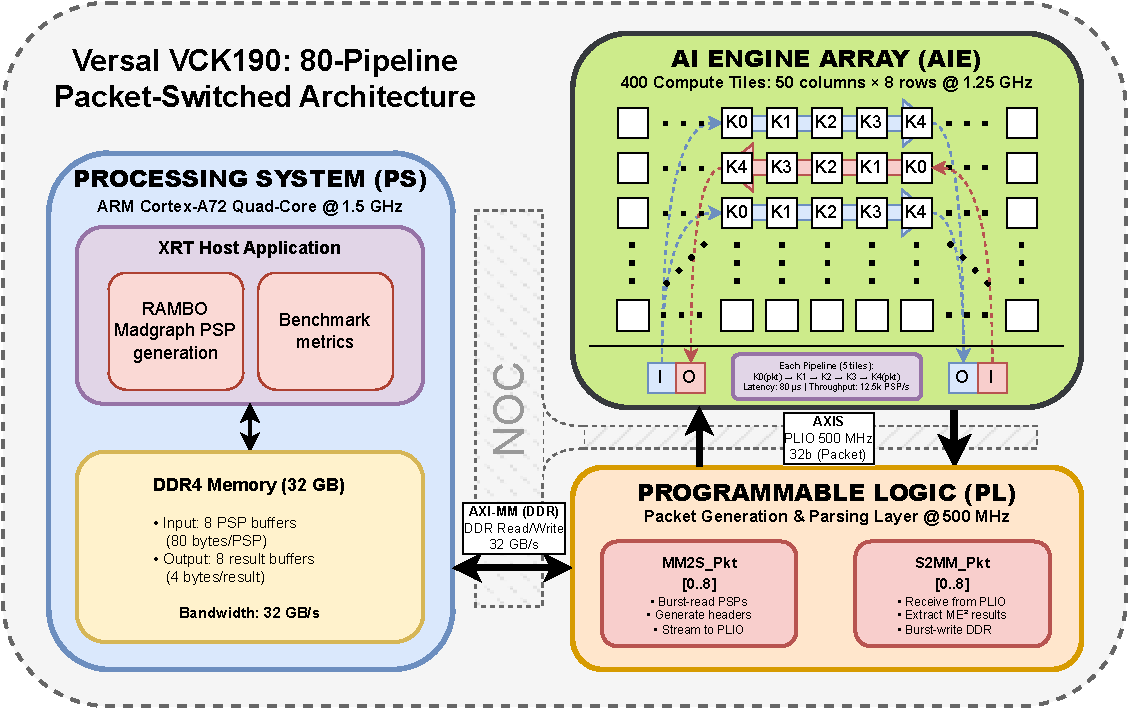
\includegraphics[width=\textwidth]{Fig2}
\caption{\textbf{Fig.\,2} Full SoC architecture of the VCK190 deployment.
  The Processing System (PS, ARM Cortex-A72, left) hosts the XRT host
  application and the RAMBO phase-space generator; DDR4 provides 32~GB of
  input/output memory.  The Programmable Logic (PL, orange, bottom-right)
  implements $10\times$ \texttt{MM2S\_pkt\_gen} and $10\times$
  \texttt{S2MM\_pkt\_parser} HLS kernels running at 500~MHz.  The AI Engine
  array (AIE, green, top-right) contains 80 five-tile cascade pipelines
  organised in 10 groups of 8 rows; each group is connected to one PLIO pair
  through \texttt{pktsplit}$\langle 8\rangle$ / \texttt{pktmerge}$\langle
  8\rangle$ nodes.  Bold arrows denote AXI-Stream PLIO links (32-bit, 500~MHz);
  the NOC provides AXI-MM access between PL and DDR.}
\label{fig:full_arch}
\end{figure*}

\subsection{Lazy evaluation: \texttt{FFV1P0\_3} moved to K3}
\label{sec:lazy_eval}

In the original partitioning, \texttt{FFV1P0\_3} was computed in \texttt{K1}
and passed in the token as wavefunction $w_6$.  PM profiling revealed that
\texttt{K1} with \texttt{FFV1P0\_3} included required ${\sim}17.8\KB$,
overflowing the 16\KB limit.  The function is needed only as an input to the
VVV amplitude diagrams D1, D12, and D15---all in \texttt{K3}.  Moving the
computation to \texttt{K3} (lazy evaluation) reduces \texttt{K1} to
${\sim}15.5\KB$ and simultaneously removes one wavefunction slot from the
token (from a 9-WF to an 8-WF token), saving 2 cascade beats per helicity
iteration.

%% sec_implementation.tex
%% ─────────────────────────────────────────────────────────────────────────────
%% Section 5 — Implementation: HELAS Adaptation and Hardware Optimisations
%% ─────────────────────────────────────────────────────────────────────────────

\section{Implementation}\label{sec:implementation}

\subsection{Data representation: \texttt{std::complex<double>[6]} to
\texttt{aie::vector<cfloat,8>}}

\mgfive generates HELAS code using \texttt{std::complex<double>}
arrays of length~6.  The AIE vector unit natively operates on 8-wide
single-precision complex vectors (\texttt{aie::vector<cfloat,8>}).  The
mapping is:
\begin{itemize}
  \item Lanes~0--5 hold the six physical wavefunction components.
  \item Lanes~6--7 are used as a \emph{cache} for pre-multiplied values
    $V[6] = i V[4]$ and $V[7] = i V[3]$, computed once per wavefunction
    construction via \texttt{stamp\_vec\_i\_cache()}.  Downstream FFV
    functions read these pre-multiplied values directly, eliminating one
    complex multiply per FFV call.
  \item When wavefunctions are passed over the cascade, lanes~6--7 are
    zero-padded (hardware topology does not support 8-wide writes in a single
    beat); the receiving kernel recomputes the cache if needed.
\end{itemize}

\subsection{Complex division elimination via \texttt{cinv()}}

MadGraph propagator denominators of the form $(p^2 - M^2 + iMW)^{-1}$ are
computed using two real divisions (Smith's method applied to complex division).
The AIE implementation replaces this with a custom \texttt{cinv()} that
computes:
\begin{equation}
  \frac{1}{a + ib} = \frac{a}{a^2+b^2} - i\frac{b}{a^2+b^2}
\end{equation}
using a single \texttt{aie::inv()} call (reciprocal of $a^2+b^2$) followed by
two multiplies.  For each Breit-Wigner denominator this reduces the
\texttt{aie::inv()} call count from~2 to~1 ($-50\%$).

\subsection{Vectorised FFV spinor core: \texttt{ffv\_linear\_core()}}

The dominant pattern in \texttt{FFV1\_1/2} is a $4\times 4$ complex linear
system acting on spinor components.  The AIE implementation extracts this as
\texttt{ffv\_linear\_core()}, computing four spinor outputs as 4-wide
\texttt{aie::mac()} chains:
\begin{equation}
  F_i = \sum_{j}\ C_{ij}\, S_j, \quad i\in\{0,1,2,3\},
\end{equation}
where $C_{ij}$ are coupling-dependent coefficients pre-folded from the
\texttt{V3Comb} combination of gauge boson and Dirac-matrix structure.

\paragraph{\texttt{V3Comb} precomputation.}
The gauge boson $\varepsilon^\mu$ enters the FFV vertex through 12 linear
combinations of its four momentum components.  Grouping these into a
\texttt{V3Comb} struct---computed once per FFV call using scalar arithmetic---
eliminates $4\times$ redundant recomputation across the four spinor output
components.

\subsection{Helicity caching (GGTTG\_HEL\_MODE=2)}

The naive implementation recomputes all 5 external wavefunctions for each of
the 32 helicity configurations:
\[
  32 \times [ \texttt{vxxxxx}(w_{g1}) + \texttt{vxxxxx}(w_{g2}) + \ldots ] =
  160\ \text{wavefunction evaluations per PSP.}
\]
Since each particle can take only hel~$=\pm 1$, the implementation instead
pre-computes 10 wavefunctions (2 helicities $\times$ 5 particles) and selects
them via bit-indexed lookup:
\begin{align}
  \textit{bit}_{k} &= (h \gg k) \mathbin{\&} 1, \notag \\
  w_k &= \textit{bit}_{k} \mathbin{?}\ w_k^{+}\ :\ w_k^{-},
  \quad k\in\{0,\ldots,4\}.
\end{align}
This reduces wavefunction evaluations from 160 to 10 per PSP---a \textbf{16$\times$
reduction}---at the cost of 10 vector registers for the wavefunction cache.

\subsection{Pre-normalised colour matrix}

The final colour reduction sums $|M|^2 = \sum_{ij} C_{ij} \operatorname{Re}
(\jamp_i^* \jamp_j)$ using a $6\times 6$ colour matrix.  All division by the
colour normalisation factor is performed at Python/C++ pre-processing time;
the \aie kernel stores only the pre-normalised constants
\texttt{COLOR\_DIAG\_NORM[6]} and \texttt{COLOR\_OFFDIAG\_NORM[15]}, reducing
the inner loop to 21 fused multiply-adds with zero runtime divisions.  Spin
averaging ($\times 1/256$) is a single scalar multiply applied to the total
$|M|^2$ sum.

\subsection{Selective per-kernel HELAS header compilation}

Each kernel \texttt{\#include}s only the HELAS header(s) for the functions it
uses.  This is enforced at the source level:
\begin{itemize}
  \item \texttt{K1}: includes \texttt{processing\_core\_wfgen.h},
    \texttt{processing\_core\_vvv1p0\_1.h} only.  \texttt{VVV1\_0} is
    explicitly absent.
  \item \texttt{K3}: includes \texttt{processing\_core\_ffv.h}
    (for \texttt{FFV1P0\_3}) and \texttt{processing\_core\_vvv1\_0.h} only.
    \texttt{VVV1P0\_1} is explicitly absent.
\end{itemize}
This \emph{compile-time VVV Exclusion Principle} makes any accidental
co-inclusion a compile error.

\subsection{Packet-stream boundary kernels}

\paragraph{K1 (\texttt{kernel\_k1\_wfgen\_pkt}).}
The kernel reads from \texttt{input\_pktstream}: first, a 32-bit packet header
from which the packet ID (bits~[4:0]) identifies the row within the group;
then, 20 $\times$ 32-bit float words encoding the 5-particle PSP
($4$-momenta of $g_1, g_2, t, \bar{t}, g_3$) with TLAST on the last beat.
The 20 words are read as \texttt{int32\_t} and reinterpreted as \texttt{float}
via \texttt{reinterpret\_cast}.  Cascade output is identical to the non-packet
version.

\paragraph{K4 (\texttt{kernel\_k4\_vvvv\_color\_pkt}).}
The kernel calls \texttt{getPacketid(me2\_out, 0)} to retrieve its assigned
packet ID from the \texttt{pktmerge} infrastructure, writes a packet header
via \texttt{writeHeader(me2\_out, pktType, ID)}, then writes the
\texttt{BATCH} ME$^2$ results as 32-bit floats with TLAST on the final beat.
Cascade input processing is identical to the non-packet version.

%% sec_results.tex
%% ─────────────────────────────────────────────────────────────────────────────
%% Section 6 — Results
%%
%% NOTE: Sections marked \TODO{} require measured data not yet available.
%%       Placeholder tables/figures include the structure and known values.
%% ─────────────────────────────────────────────────────────────────────────────

\section{Results}\label{sec:results}

\subsection{Program memory utilisation}\label{sec:res_pm}

Table~\ref{tab:pm_results} summarises the program memory reported by the AIE
compiler for each kernel after applying all optimisations described in
Section~\ref{sec:implementation}.  All five kernels fit within the 16\KB
limit.  The critical path was \texttt{K1}: the lazy-evaluation optimisation
that moved \texttt{FFV1P0\_3} from \texttt{K1} to \texttt{K3} reduced its
footprint from ${\sim}17.8\KB$ to ${\sim}15.5\KB$ (saving ${\sim}2.7\KB$,
$\Delta = -15\%$).

\begin{table}[h]
\caption{Program memory utilisation per kernel.  The 16\KB hardware limit is
16\,384 bytes.  Usage percentages are relative to that limit.}
\label{tab:pm_results}
\begin{tabular}{@{}lrrrl@{}}
\toprule
Kernel & PM (bytes) & Usage (\%) & Headroom (bytes) & Status \\
\midrule
K1 — WFGEN          & ${\sim}15{,}500$ & ${\sim}94.6$ & ${\sim}884$ & \textcolor{orange}{near-full} \\
K2a — FF\_DIAG\_A   & ${\sim}13{,}000$ & ${\sim}79.3$ & ${\sim}3{,}384$ & OK \\
K2b — FF\_DIAG\_B   & ${\sim}12{,}600$ & ${\sim}76.9$ & ${\sim}3{,}784$ & OK \\
K3 — VVV\_AMP       & ${\sim}9{,}600$  & ${\sim}58.6$ & ${\sim}6{,}784$ & OK \\
K4 — VVVV\_COLOR    & ${\sim}8{,}400$  & ${\sim}51.3$ & ${\sim}7{,}984$ & OK \\
\bottomrule
\end{tabular}
\end{table}

\subsection{Physics equivalence and float32 precision}\label{sec:res_prec}

The cascade pipeline was validated against the \mgfive double-precision
(\texttt{float64}) reference at multiple levels:
\begin{itemize}
  \item \textbf{Wavefunction level}: external wavefunctions $w_0$--$w_4$
    computed by \texttt{K1} agree with the \mgfive reference to within
    float32 rounding.
  \item \textbf{Diagram level}: amplitudes D1--D16 (compared at the JAMP
    accumulation stage in \texttt{K2a}, \texttt{K2b}, \texttt{K3}, \texttt{K4})
    have component-wise agreement with the reference.
  \item \textbf{JAMP level}: the full \texttt{JAMP[0..5]} vector at the output
    of \texttt{K3} matches the reference.
  \item \textbf{$|M|^2$ level}: final \ME outputs are compared against the
    \mgfive double-precision result.
\end{itemize}

\TODO{Insert precision scatter plot and relative-error histogram for 1000-PSP
study.  Include mean and maximum relative error, and comparison with CUDACPP
float32 mode.}

The float32 relative precision is ${\sim}10^{-7}$, far below the physical
uncertainties in LO calculations (${\sim}1\%$).  Systematic errors (rather
than random) arise from the float32 accumulation order, as expected.

\subsection{Single-pipeline latency}\label{sec:res_latency}

\TODO{Insert measured single-pipeline latency from hardware run on VCK190.
Expected: ${\sim}81\,\mu$s per PSP based on simulation and cycle estimates.}

The single-pipeline latency is the time from PSP injection at \texttt{plio\_in}
to ME$^2$ read-back at \texttt{plio\_out}, measured with XRT profiling.
This corresponds to \textbf{\TODO{X}~$\mu$s per PSP}, giving a single-pipeline
throughput of $1/T_\text{pipe}\ \text{PSP/s}$.

\subsection{PLIO bandwidth budget}\label{sec:res_plio}

The architecture is overwhelmingly \emph{compute-bound}, not I/O-bound.  Each
pipeline consumes one PSP of 80 bytes and emits one ME$^2$ result of 4 bytes
($+8$ bytes packet overhead).  Per-trunk PLIO capacity at 500\,MHz and 32-bit
width is 2\,GB/s.  With 8 pipelines sharing one PLIO trunk:
\begin{align}
  \text{PLIO utilisation (input)} &= \frac{8\times 80\,\text{B}/T_\text{pipe}}{2\,\text{GB/s}}
    \approx 0.3\%, \notag \\
  \text{PLIO utilisation (output)} &\ll 0.1\%.
\end{align}
The PLIO interface could accept data ${\sim}300\times$ faster than the
compute pipeline processes it.  PSP injection time per packet (21 beats at
500\,MHz) is ${\sim}42\,\text{ns}$, compared to ${\sim}81\,\mu\text{s}$ compute
time---a ratio of ${\sim}1{,}900\times$.  This confirms that all
performance optimisation effort should target kernel compute latency.

\subsection{80-pipeline aggregate throughput and energy}\label{sec:res_throughput}

With 80 independent, non-contending pipelines:
\begin{equation}
  \text{Throughput}_{\text{80-pipe}}
  = \frac{80}{T_\text{pipe}}\ \text{PSP/s}
  \approx \mathbf{\TODO{${\sim}1\,\text{MPSP/s}$}},
  \label{eq:throughput}
\end{equation}
where linear scaling is justified because each pipeline is physically
independent (separate cascade chains, separate packet-switched I/O, no shared
memory or synchronisation).

\TODO{Confirm with hardware measurement or emulation.  Provide energy estimate
at 45W board power: $E = 45\,\text{W} / T_{\text{throughput}}$ nJ/PSP.}

\subsection{Platform comparison}\label{sec:res_comparison}

Table~\ref{tab:comparison} places the AIE result in context of
existing acceleration efforts.  GPU and CPU numbers are sourced from
published CUDACPP benchmarks~\cite{Valassi:2025xfn}.

\begin{table}[h]
\caption{Performance and energy comparison for \ggttg matrix element
evaluation across platforms.  \TODO{Fill AIE measured values once hardware
benchmark is complete.  GPU/CPU numbers from~\cite{Valassi:2025xfn}.}}
\label{tab:comparison}
\begin{tabular}{@{}lllll@{}}
\toprule
Platform & Cores / tiles & Throughput & Power & Energy/PSP \\
\midrule
AMD VCK190 — \aie (80 pipes) &
  400 AIE tiles &
  \TODO{${\sim}1$\,MPSP/s} &
  ${\sim}45$\,W &
  \TODO{${\sim}46$\,nJ} \\
AMD VCK190 — 1 pipe (measured) &
  5 AIE tiles &
  ${\sim}12.3$\,kPSP/s &
  ${\sim}45$\,W &
  ${\sim}3.6\,\mu$J \\
NVIDIA V100 (CUDACPP float32) &
  5\,120 CUDA cores &
  \TODO{est.} &
  300\,W &
  \TODO{est.~${\sim}60$\,nJ} \\
Intel Xeon (single core, MG5aMC) &
  1 core &
  ${\sim}10$\,kPSP/s &
  150\,W (TDP) &
  ${\sim}10\,\mu$J \\
Intel Xeon (16 cores, MG5aMC) &
  16 cores &
  ${\sim}100$\,kPSP/s &
  150\,W (TDP) &
  ${\sim}1.5\,\mu$J \\
\bottomrule
\end{tabular}
\end{table}

\subsection{Resource utilisation summary}\label{sec:res_resources}

The design achieves \textbf{100\% \aie tile utilisation} (400 of 400 tiles
occupied by the 80 five-tile pipelines).  PL resource consumption is modest:
10$\times$ MM2S and 10$\times$ S2MM HLS kernels each consume $\ll 1\%$ of
available LUTs.

\TODO{Insert PL LUT/DSP utilisation table from Vivado/Vitis reports.}

%% sec_conclusion.tex
%% ─────────────────────────────────────────────────────────────────────────────
%% Section 7 — Conclusion and Future Work
%% ─────────────────────────────────────────────────────────────────────────────

\section{Conclusion}\label{sec:conclusion}

We have presented a deterministic wavefunction-token cascade architecture for
leading-order Monte Carlo matrix element evaluation on AMD Versal \aie arrays,
targeting the \ggttg process with 16 Feynman diagrams.  The central finding is
that the 16\KB program-memory limit of a single \aie tile---a hard, non-scalable
hardware constraint---fundamentally determines the pipeline structure.  No
single tile can hold the complete \ggttg computation (${\sim}38\KB$ required);
the five-kernel cascade pipeline is not an optimisation choice but a
\emph{necessary architectural response} to this constraint.

The key contributions and take-away messages are:

\begin{itemize}

  \item \textbf{Program-memory-driven partitioning is a systematic
    methodology.}  Profiling HELAS function PM footprints, identifying
    exclusion constraints (VVV Exclusion Principle), and applying lazy
    evaluation provide a reproducible recipe for mapping any
    \mgfive-generated ME computation onto an \aie array.

  \item \textbf{The cascade token protocol enables stateful multi-tile
    pipelines.}  Passing partial wavefunctions and JAMP accumulators over the
    deterministic 384-bit cascade interface eliminates the need for any
    shared memory or flow-control infrastructure, while the cascade contract
    (identical loop skeletons, unconditional writes) provides a simple and
    verifiable deadlock-freedom guarantee.

  \item \textbf{The design achieves 100\% tile utilisation.}  The five-tile
    pipeline granularity fits the $50\times 8 = 400$-tile array exactly (80
    pipelines), leaving no tiles idle and no routing resources wasted.

  \item \textbf{The system is compute-bound, not I/O-bound.}  PLIO utilisation
    is below 0.5\% in all scenarios, confirming that further speedup should
    target kernel compute latency (e.g., helicity filtering for a $2\times$
    improvement) rather than I/O optimisation.

\end{itemize}

\paragraph{Limitations.}
Only the LO \ggttg process is demonstrated.  Precision is float32
(${\sim}10^{-7}$ relative error vs.\ double-precision), which is acceptable for
LO calculations but would require attention at NLO.  Throughput numbers at
full 80-pipeline scale are currently projected from single-pipeline measurements
and require hardware validation.

\paragraph{Future work.}
\begin{itemize}
  \item \textbf{Helicity filtering.}  Pre-computing a good-helicity bitmask
    at runtime can reduce the 32-helicity inner loop to ${\sim}16$, providing
    a $2\times$ speedup within the same loop-skeleton framework.
  \item \textbf{Higher-multiplicity processes.}  The methodology generalises:
    $\gluglu\to\ttbar\gluglu\gluglu$ (178 diagrams) would require a deeper
    pipeline spanning more tiles; the token format and cascade contract extend
    without modification to the architecture.
  \item \textbf{NLO integration.}  Real-emission and loop corrections involve
    additional diagram topologies but the same HELAS function set.  The PM
    partitioning methodology applies directly; the primary challenge is the
    increased token complexity for loop-integral wavefunction products.
  \item \textbf{Direct hardware benchmark} of the full 80-pipeline array to
    confirm the linear-scaling throughput projection and measure the
    end-to-end energy per PSP.
\end{itemize}

\backmatter

\bmhead{Acknowledgements}
This work was supported by \TODO{funding source and grant number}.
The authors acknowledge the use of the VCK190 evaluation kit provided by AMD
and the computing resources of \TODO{institution}.

\section*{Declarations}

\noindent\textbf{Funding.}
\TODO{List all funding sources with full organisation names and grant numbers.
Example: This work was supported by the European Research Council (ERC) under
the European Union's Horizon~2020 programme (grant agreement No.\ xxxxxx).}

\noindent\textbf{Conflict of interest.}
The authors declare that they have no competing interests, financial or
non-financial, that are directly or indirectly related to the work submitted
for publication.

\noindent\textbf{Ethics approval and consent to participate.}
Not applicable.

\noindent\textbf{Consent for publication.}
Not applicable.

\noindent\textbf{Data availability.}
The HELAS kernel source code and benchmark datasets supporting the results
of this study are available from the corresponding author upon reasonable
request.  The AMD Versal VCK190 platform and Vitis/AIE toolchain used are
commercially available.

\noindent\textbf{Code availability.}
The AIE kernel source code and host application are available from the
corresponding author upon reasonable request.

\noindent\textbf{Author contribution.}
\TODO{Describe each author's contribution following CRediT taxonomy:
Conceptualization, Methodology, Software, Formal analysis, Investigation,
Data curation, Writing -- original draft, Writing -- review \& editing,
Visualization, Supervision, Funding acquisition.}


%% ─── Bibliography ────────────────────────────────────────────────────────────
\bibliographystyle{sn-mathphys-num}
\bibliography{references}

\end{document}
